\providecommand{\main}{../..}  % define path to bib location for subfiles
\documentclass[../../main.tex]{subfiles}
\begin{document}
\onlyinsubfile{
\setcounter{chapter}{0}
}
\notinsubfile{}
\chapter{Inleiding}\label{chap:H1}
\marginpar{
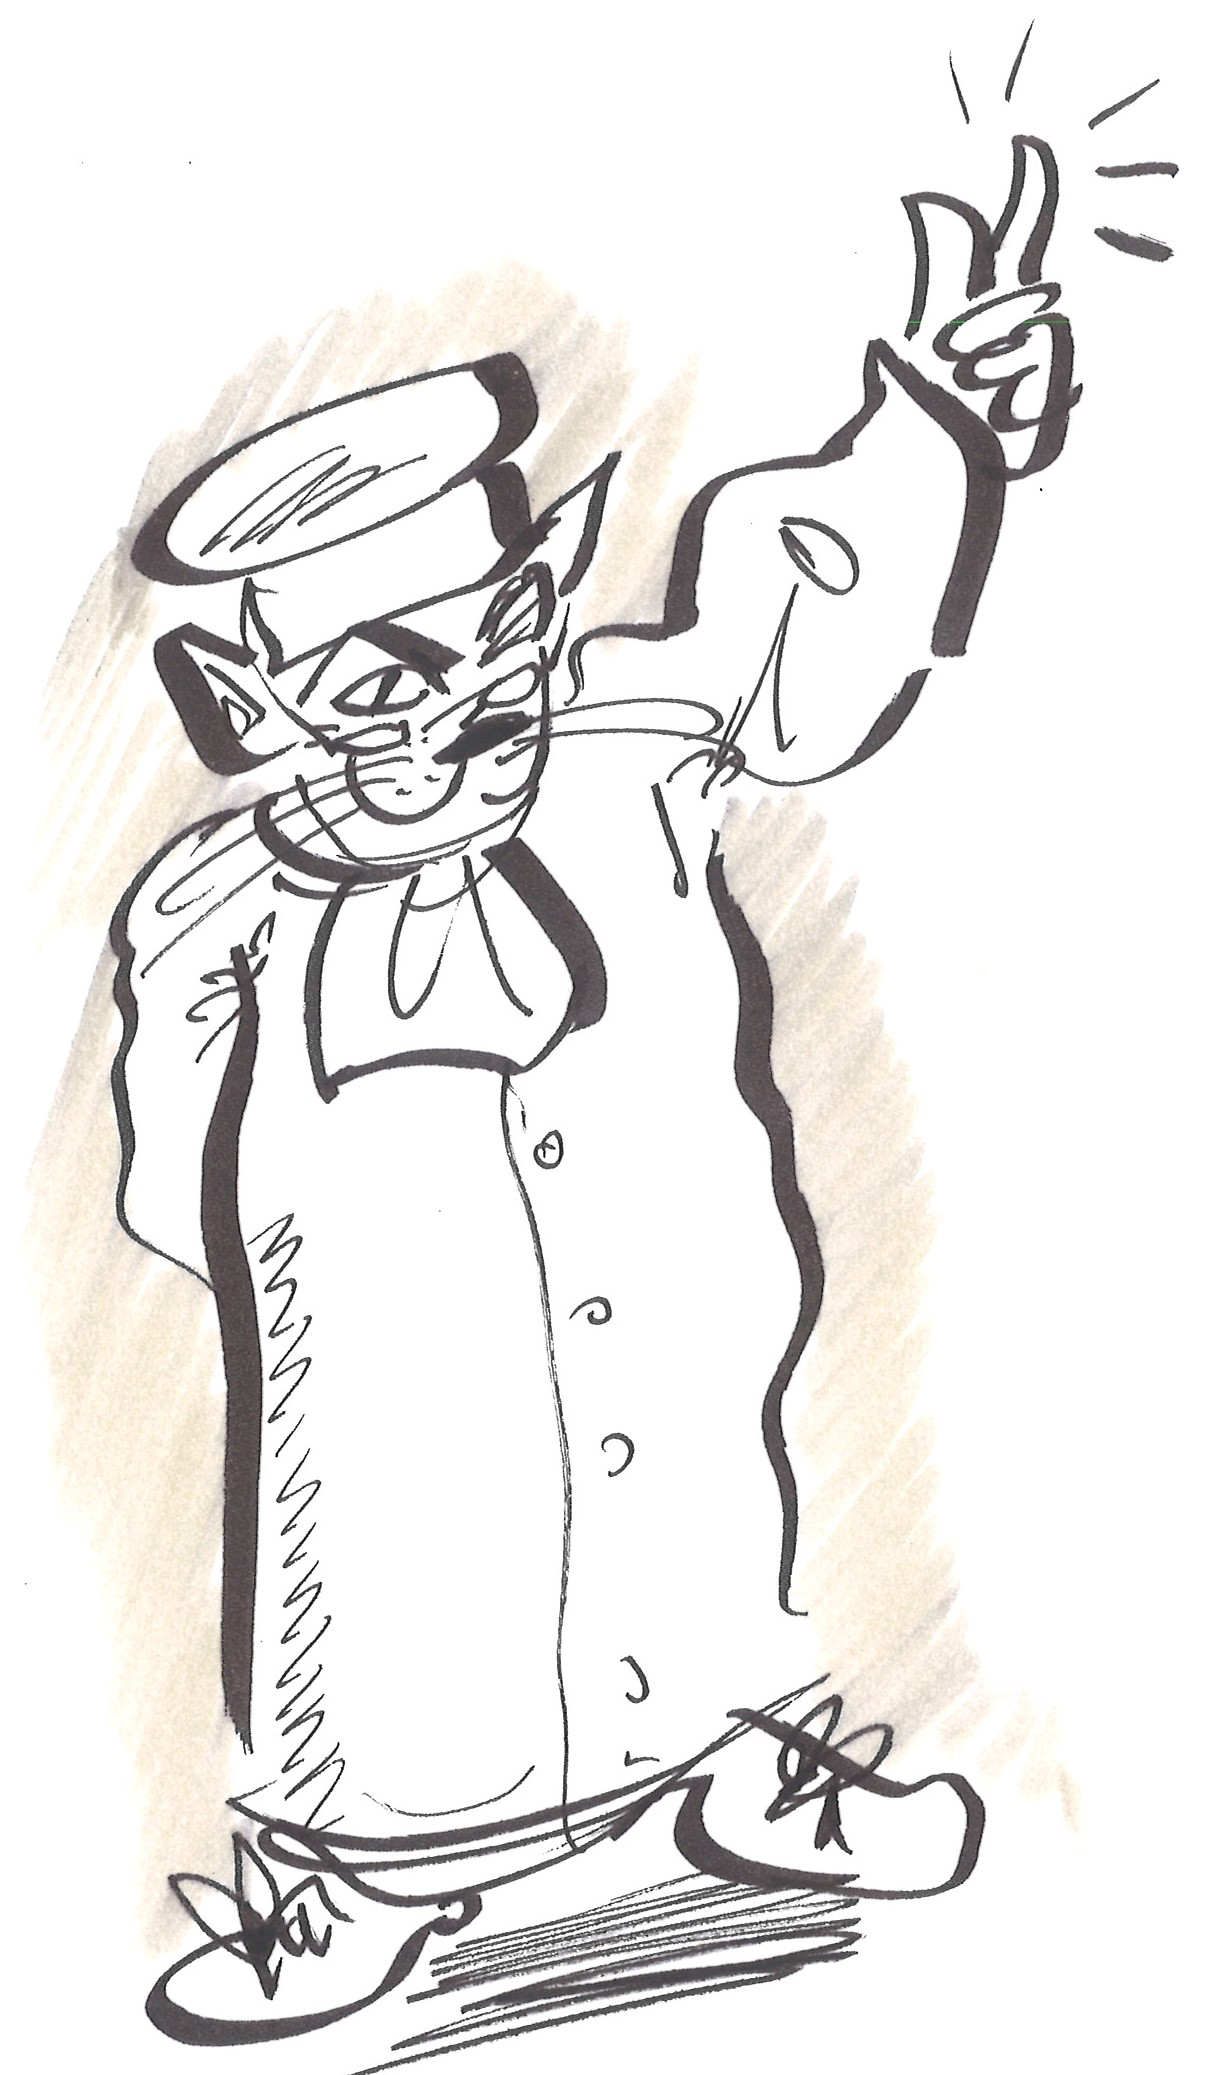
\includegraphics[width=0.4\textwidth]{./img/prof1.jpg}
}

\section{Inleiding}
Voor je ligt de NLT module Kansen met Quantum. De module behandelt de ontwikkeling van de quantumcomputing, een technologie die voortvloeit uit de quantumtheorie. Deze theorie is inmiddels meer dan 100 jaar oud, en bleek de sleutel tot het begrip van de materie op de kleinste schaal. Op die schaal zit de wereld werkelijk anders in elkaar dan onze vertrouwde,  klassieke, Newtoniaanse ervaringswereld. Je hoort vaak uitspraken als 'deeltjes kunnen op twee verschillende plaatsen tegelijkertijd zijn', of 'deeltjes kunnen reizen als golf en worden weer gedetecteerd als deeltje'. 
De hoofdlijnen van de theorie zijn in de eerste helft van de twintigste eeuw beschreven. De theorie opende een nieuwe wereld en heeft tot veel uitvindingen geleid, zoals bijvoorbeeld de transistor. Bij het vak natuurkunde komt deze '1.0 versie' van quantumtheorie uitgebreid aan de orde. 

De quantumtheorie is niet intu\"itief. Zo kunnen deeltjes verdeeld zijn over meerdere toestanden. Erwin Schr\"odinger beschreef dit in een gedachtenexperiment met een kat. Deeltjes kunnen ook met elkaar verstrengeld zijn. Op grote afstand kan een verandering in de toestand in het ene deeltje een verandering van het andere deeltje veroorzaken. Einstein~\cite{Einstein1935} noemde het een paradox.  Volgens hem  moesten er nog onderliggende variabelen zijn om de theorie compleet te maken.
\marginpar{\vspace{-1cm}\footnotesize{In de 'klassieke' wereld kunnen deeltjes geen eigenschappen delen op grote afstand (alleen \textit{local}) en je kunt alleen iets zeggen over een deeltje als je het meet (\textit{realism}). In de quantumwereld geldt deze beperking niet.}}

In 1982 leverde Alain Aspect een acceptabel bewijs voor het falen van Einstein's \textit{\textit{local realism}}: eigenschappen van deeltjes kunnen inderdaad over grote afstand gekoppeld zijn en je kunt geen uitspraak doen over de toestand van een deeltje als je het niet meet~\cite{mermin1985moon}.

In de tweede helft van de twintigste eeuw groeide het besef dat ook dit deel van de  quantumtheorie gebruikt zou kunnen worden voor een hele reeks van toepassingen. Een tijdlijn over de ontwikkeling van quantumcomputing~\cite{timeline2021} zet de belangrijkste ontdekkingen vanaf 1960 op een rijtje. Vanaf de jaren 1980 is een versnelling te zien. Richard Feynman is een van de sleutelfiguren. Hij bracht naar voren dat quantumprocessen het best gesimuleerd kunnen worden op een computer waarvan de werking zelf gebaseerd is op quantumverschijnselen. Klassieke informatieverwerking is gebaseerd op bits die de waarden 0 of 1 kunnen aannemen. Quantumbits of kortweg qubits kunnen tegelijkertijd in \textit{superpositie} van 0 en 1 zijn. En wat dat precies betekent? Ja, daar gaat deze module over. 



\begin{center}
\mbox{\begin{minipage}{.6\textwidth}
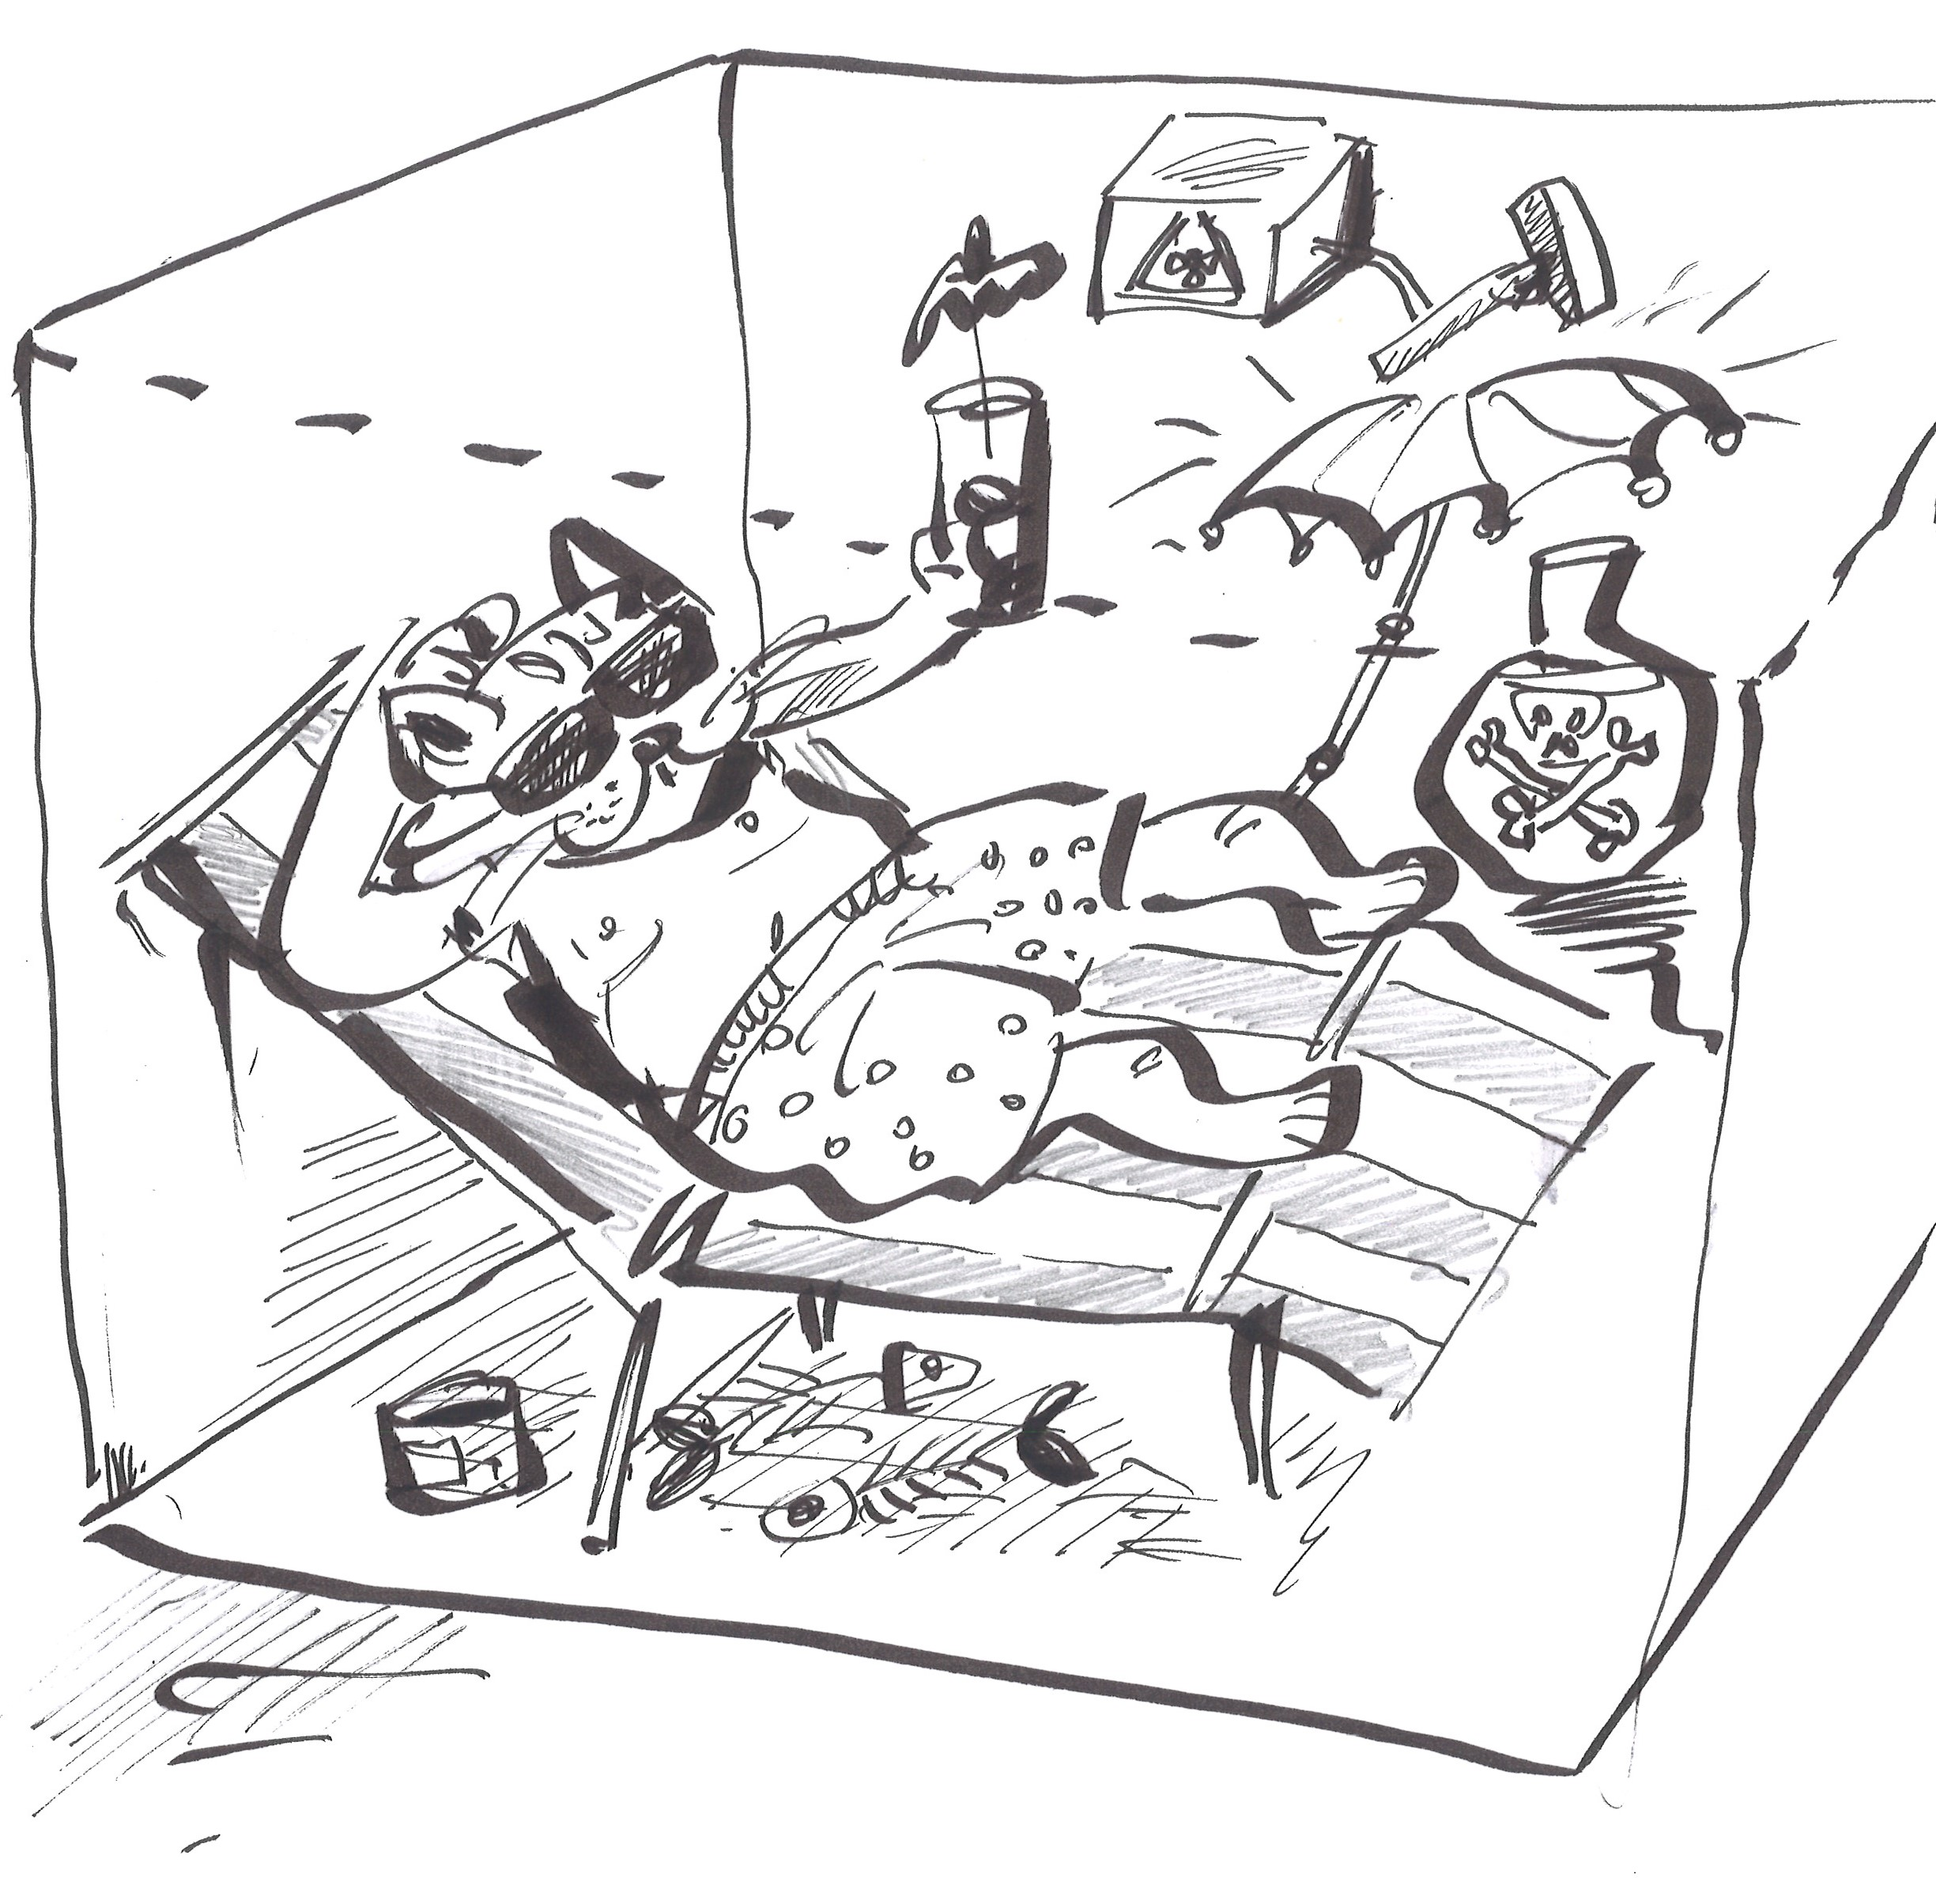
\includegraphics[width=\textwidth]{./img/4634_003inthebox.jpg}
\end{minipage}}%
\hfill%hier geen extra linefeeds!!!
\mbox{\begin{minipage}{.8\textwidth}
\small{Wat nou dood of levend Erwin? Ik ben in superpositie!}\label{fig:inthebox}
\end{minipage}}
\end{center}


De kracht van quantumcomputers is dat ze wezenlijk andere dingen kunnen dan klassieke computers. Met de juiste voorbereiding kunnen ze bijvoorbeeld met \'e\'en qubit een probleem oplossen waar een klassieke computer twee bits nodig heeft. Dit staat bekend als condensed coding of het orakel van Deutsch. Het stelt misschien nog niet veel voor maar als \textit{proof of principle} is het een belangrijke stap. In een keuze-opdracht kun je het algoritme hiervoor ontdekken. Ook is het mogelijk (je gaat dit in deze module ontdekken) om de toestand van een qubit te teleporteren, een belangrijke stap in de ontwikkeling van quantum-beveiligde communicatie. Er is een quantumalgoritme dat het zoeken in een ongesorteerde lijst versnelt. In een ouderwets telefoonboek staan de telefoonnummers naast een alfabetisch gesorteerde lijst met namen. Het is heel makkelijk om het nummer bij een naam te vinden, maar de nummers staan in willekeurige volgorde (ongesorteerd). Als je een naam bij een nummer wilt vinden  tref je het nummer nadat je gemiddeld de helft van het boek hebt doorgeworsteld. Als het telefoonboek twee keer zo dik is duurt het zoeken ook twee keer zo lang. Het quantum-algoritme van Lov Grover (1996)versnelt deze zoekopdracht kwadratisch. Als het telefoonboek negen keer zo dik is, duurt het zoeken drie keer zo lang. Voor lange lijsten levert dat een enorm voordeel.

 %31*37=1137%29*53=1537
Een belangrijke doorbraak is de ontdekking van het factorisatie-algoritme van Peter Shor (1994). Factoriseren is het ontbinden van getallen in priemfactoren. Het coderingssysteem RSA, dat de basis vormt voor o.a. onze banktransacties is gebaseerd op de aanname dat het ontbinden in priemfactoren van een groot getal (denk aan getallen van 4000 cijfers) veel rekentijd kost. Het is niet onmogelijk, maar klassieke algoritmen doen hier veel te lang over (eeuwen of langer). Het algoritme van Peter Shor kan het ontbinden aanzienlijk versnellen als de langzaamste stap draait op een quantumcomputer. Encryptie volgens het RSA systeem is dus met quantumcomputing te kraken. Dit heeft enorme maatschappelijke gevolgen. Gelukkig geven quantumcomputers ook de oplossing: er worden nieuwe post-quantum encryptiesystemen ontwikkeld. 

Peter Shor's algoritme kwam niet uit het niets. In dit \hrefqr[0cm]{https://www.youtube.com/watch?v=6qD9XElTpCE&list=RDLV6qD9XElTpCE&start_radio=1&t=1553s&ab_channel=Qiskit}{filmpje} (tussen ongeveer 8:50-14 minuten) vertelt hij hoe hij vanaf 1991 tot zijn ontdekkingen is gekomen. Hij noemt daarbij telkens met wie hij samenwerkt. Zo werkt wetenschap.

De opkomst van de quantumcomputer schept onrust bij banken, het verzekeringswezen en de wereld van de tech-giganten zoals Google, Amazon en IBM. Zij  begrijpen dat quantumtechnologie de wereld ingrijpend kan gaan veranderen. En wie te laat komt mist de boot. Er worden nu miljarden ge\"investeerd door deze bedrijven en overheden. In Nederland is in 2019 de Nationale Agenda Quantumtechnologie~\cite{agenda2019} opgesteld. Daarin wordt een flink aantal gebieden genoemd waarin de quantumtechnologie een rol kan gaan spelen. We noemen enkele voorbeelden:

\begin{itemize}
\item Cryptografie: behalve gevaren voor de bestaande versleutelingstechnieken biedt de quantumcomputer ook een mogelijkheid om communicatie te beveiligen. In de module behandelen we het  BB84-protocol~\cite{BENNETT20147}. 
\item Rekensnelheid: niet alleen bij het algoritme van Shor is de quantumcomputer superieur aan de klassieke computer. Er is in 2009 een algoritme opgesteld om een stelsel lineaire vergelijkingen sneller te kunnen oplossen. Ook wordt gewerkt aan snellere algoritmes ten behoeve van optimalisatieproblemen. Als toepassing worden genoemd: klimaatvoorspellingen, doorrekenen van modellen op het gebied van waterhuishouding, modelberekeningen uit de financiële wereld, (medische) beeldvorming, proces-optimalisatie etc.

\item Simulaties: De meest voor de hand liggende toepassingen liggen in het simuleren van grote moleculen zoals in de farmacie. Een ander voorbeeld is het maken van kunstmest. De grondstof voor kunstmest is ammoniak ($NH_3$). Dat wordt nu gemaakt volgens het Haber-Bosch proces. Dit proces vindt plaats bij hoge temperatuur en druk en kost enorm veel energie. Bacteri\"en in de wortels van vlinderbloemigen kunnen stikstof uit de lucht ($N_2$) enzymatisch, bij kamertemperatuur en druk, omzetten in ammoniak. Dit proces kost veel minder energie. Zij gebruiken hiervoor een enzym (FeMoCo) waarvan de werking nog niet begrepen is. Omdat dit een relatief klein enzym is zouden quantumcomputers al op korte termijn een bijdrage kunnen leveren aan de oplossing van het kunstmest probleem.
Zonder dat er nog een quantumcomputer is hebben al veel vakgebieden nagedacht over toepassingen. Voor een overzicht zie tabel~2 in~\cite{Georgescu2014}.
\end{itemize}

\subsection*{Opbouw en leerdoelen}
De module bestaat uit twee delen. In het eerste deel bouwen we ons begrippenapparaat
op, in het tweede deel passen we onze kennis toe in praktische opdrachten. Het eerste deel bestaat uit drie hoofdstukken, met opgaven en werkbladen. Aan het eind van ieder hoofdstuk staan de leerdoelen samengevat. In hoofdstuk~\ref{chap:H1} beginnen we met een korte inleiding op het onderwerp en maken we kennis met enkele belangrijke begrippen en fenomenen door zelf te experimenteren met licht. Om de vergelijking te maken met een quantumcomputer begint hoofdstuk~\ref{chap:H2} met een korte uitleg over hoe een klassieke computer werkt. We onderbouwen ons wiskundig begrippenapparaat met een model. Het hoofdstuk eindigt met een eisenlijst waaraan een quantumcomputer moet voldoen. In hoofdstuk~\ref{chap:H3} behandelen we de bouwblokken (poorten) van quantumcomputers. We zien dat die echt anders zijn. We combineren de poorten in een algoritme dat je echt niet op een klassieke computer kunt uitvoeren: teleportatie. We sluiten het hoofdstuk af met een blik op de toekomst. Na dit hoofdstuk volgt een toets.

Het tweede deel (hoofdstuk~\ref{chap:H4}) is een verzameling praktische keuze-opdrachten.
In dit deel onderzoek je in samenwerkingsverband een aspect van quantumcomputing; je onderzoekt een algoritme, je verdiept je in wiskunde D, onderzoekt een technisch aspect of je denkt na over de maatschappelijke consequenties. Er is ook de mogelijkheid om dit deel in te vullen met een activiteit aangeboden door \'e\'en van de universiteiten bij jou in de buurt. Wanneer je deze module hebt afgesloten, hopen we dat je een goed beeld hebt gevormd over wat deze technologie in de toekomst voor jou en de maatschappij kan betekenen.

\section{Een experiment uit de 'oertijd'}
We starten met een experiment dat al in 1802 door Thomas Young werd uitgevoerd. Hij liet licht door smalle spleten gaan en nam golfverschijnselen waar. In werkblad~\ref{sec:wbYoung1} onderzoeken we eerst hoe licht door een enkele smalle spleet gaat, en onderzoeken we hoe twee smalle spleten elkaar be\"invloeden. We gebruiken daarna polarisatie, een eigenschap van licht die aan Young nog niet bekend was, om tot moderne inzichten in het dubbelspleetexperiment te komen. De experimenten brengen ons drie belangrijke fenomenen uit de quantumwereld: \textit{interferentie}, \textit{superpositie} en de \textit{waarneming}. Een vierde quantumeigenschap \textit{verstrengeling}, komt pas aan het eind van hoofdstuk~\ref{chap:H3} aan de orde.

\medskip
\begin{experiment}{Experiment van Young~1}
Voer het werkblad~\ref{sec:wbYoung1} uit 
\end{experiment}
%\begin{antwoord}
%\end{antwoord}

\subsection*{Polarisatie} \label{sec:eraser}
De resultaten van het experiment van Young~\ref{sec:wbYoung1} zijn een tussenstap die we even moeten onthouden. We pakken ze later weer op. Voor we er mee verder gaan, hebben we een andere eigenschap van licht nodig, polarisatie. Je kunt licht voorstellen als een \textit{transversale} golf  die zich met de lichtsnelheid voortbeweegt zoals in figuur~\ref{fig:lichtvec}. In een transversale golf is de uitwijking van een punt in een vlak loodrecht op voortgangsrichting van de golf. Lineaire polarisatiefilters laten alleen \'e\'en trillingsrichting door, de rest wordt geabsorbeerd door het filter. Ze projecteren daarmee de trilling in \'e\'en richting. 


\begin{flushleft}
\hspace*{-\marginparwidth-\marginparsep}\begin{minipage}{.65\textwidth}
\colorlet{crystal}{blue!75}
\def\zangle{-20}
\def\xangle{20}
\begin{tikzpicture}[scale=.85,x=(\xangle:0.75cm), y=(90:1cm), z=(\zangle:1.5cm),
    >=stealth, line cap=round, line join=round,
    lines/.style={gray!50, thick}, 
    axis/.style={black, thick},
    plate/.style={fill, opacity=0.875},
    markers/.style={orange, thick},
    scale=1.]
\iffalse%---circ pol
\node [yslant=tan(\zangle), above=0.25cm, align=center,font=\small] at 
    (1,1,1.5){Left Handed \\ Circularly Polarized Light};

\draw [lines] (-1,-1,0) -- (-1,1,0) -- (1,1,0) -- (1,-1, 0) -- cycle;
\draw [lines] (1,0,0) \foreach \t in {0,5,...,355}{
        -- (cos \t, sin \t, 0) } -- cycle;

\draw [lines] (1,1,0) -- (1,1,3.125);
\draw [lines] (-1,-1,0) -- (-1,-1,3.125);
\draw [axis, ->] (0,0,3.125) -- (0,0,0);

\foreach \k [evaluate={%
    \i=\k*5.625; 
    \j=\i>0 ? \i-5.625 : 0; 
    \a=90-\i; 
    \b=90-\j; 
    \c=int(mod(\k,4));}] 
    in {0,...,192}{
        \ifnum\c=0
            \draw [->] (0,0,\i/360) -- ++(cos \a, sin \a, 0);
        \fi
        \draw [red] (cos \a, sin \a, \i/360) -- (cos \b, sin \b, \j/360);
    }
\fi%---circ pol
\begin{scope}[shift={(0,0,3.125)}]%----lin pol light----

\node [yslant=tan(\zangle), above=0.25cm, align=center,font=\normalsize,scale=.4*2] at 
    (1,1,1.5){Gepolariseerd};

\begin{scope}[xscale=1.5, yscale=1.5]%----quarter waveplate
    \path [crystal!25, plate] 
        (-1,-1,0) -- (-1,1,0) -- (1,1,0) -- (1,-1,0) -- cycle;
    \path [crystal!50, plate] 
        (-1,-1,0) -- (-1,-1,-0.125) -- (-1,1,-0.125) -- (-1,1, 0) -- cycle;
    \path [crystal!75, plate] 
        (-1,1,0) -- (-1,1,-0.125) -- (1,1,-0.125) -- (1,1, 0) -- cycle;
    \node [yslant=tan(\xangle), text=crystal!50, below, font=\small] at 
        (-1.125,-1,0){muur};
\end{scope}%----quarter waveplate

\draw [markers] (0,1) -- (0,-1) (-0.5,0) -- (0.5,0);
\draw [lines] (1,1,0) -- (1,1,3);
\draw [lines] (-1,-1,0) -- (-1,-1,3);

\draw [axis] (0,0,0) -- (0,0,3);

\foreach \k [evaluate={%
    \i=\k*5.625; \j=\i>0 ? \i-5.625 : 0; 
    \a=90-\i; 
    \b=90-\j; 
    \c=int(mod(\k,4)==0 && sin \a != 0); 
    \d=int(\k+1/4);}] in {0,...,192}{
    \ifodd\d
        \ifnum\c=1
            \draw [->] (0,0,\i/360) -- ++(sin \a, sin \a, 0);
        \fi
        \draw [red] (sin \a, sin \a, \i/360) -- (sin \b, sin \b, \j/360);
    \else
        \draw [red] (sin \a, sin \a, \i/360) -- (sin \b, sin \b, \j/360);
        \ifnum\c=1
            \draw [->] (0,0,\i/360) -- ++(sin \a, sin \a, 0);
        \fi
    \fi
}
\end{scope}%----lin pol light----
\begin{scope}[shift={(0,0,6.125)}]%----unpol

\node [yslant=tan(\zangle), above=0.25cm, align=center,font=\normalsize, scale=.4*2] at 
(1,1,1.5){Ongepolariseerd};

\begin{scope}[xscale=1.5, yscale=1.5]%----linpolarizer
    \path [crystal!25, plate] 
        (-1,-1,0) -- (-1,1,0) -- (1,1,0) -- (1,-1, 0) -- cycle;
    \path [crystal!50, plate] 
        (-1,-1,0) -- (-1,-1,-0.0625) -- (-1,1,-0.0625) -- (-1,1, 0) -- 
        cycle;
    \path [crystal!75, plate] 
        (-1,1,0) -- (-1,1,-0.0625) -- (1,1,-0.0625) -- (1,1, 0) -- cycle;
    \node [yslant=tan(\xangle), text=crystal!50, below, font=\small] at 
        (-1,-1,0){Polaroid filter};
\end{scope}%----linpolarizer

\draw [markers] (-1.25,-1.25) -- (1.25,1.25);

\draw [lines] (0,1.414,0) -- (0,1.414,2);
\draw [lines] (1.414,0,0) -- (1.414,0,3);
\draw [lines] (1,1,0) -- (1,1,1);
\draw [lines] (-1,-1,0) -- (-1,-1, 0.5);
\draw [axis] (0,0,0) -- (0,0,3);

\foreach \k [evaluate={%
    \i=\k*5.625; \j=\i>0 ? \i-5.625 : 0;
    \a=90-\i; 
    \b=90-\j; 
    \c=int((mod(\k,4)==0 && sin \a != 0) || (\k==65) || (\k==129)); 
    \d=int(\k+1/4);
    \r=(\k>64) ? 1.414 : 1;
    \xa=(\k > 64) && (\k < 129) ? 0 : sin(\a)*\r;
    \xb=(\k > 64) && (\k < 129) ? 0 : sin(\b)*\r;
    \ya=(\k < 129) ? sin(\a)*\r : 0;
    \yb=(\k < 129) ? sin(\b)*\r : 0;
    }] in {0,...,192}{
        \ifodd\d
            \ifnum\c=1
                \draw [->] (0,0,\i/360) -- ++(\xa, \ya, 0);
            \fi
            \draw [red] (\xa, \ya, \i/360) -- (\xb, \yb, 
            \j/360);
        \else
            \draw [red] (\xa, \ya, \i/360) -- (\xb, \yb, 
            \j/360);
            \ifnum\c=1
                \draw [->] (0,0,\i/360) -- ++(\xa, \ya, 0);
            \fi
        \fi
    }

\draw [ultra thick, ->] (0,0,3.5) -- (0,0,3);

\end{scope}%---unpol
\end{tikzpicture}
\end{minipage}%
\hfill
\begin{minipage}{.5\textwidth}
\captionof{figure}{Ongepolariseerde fotonen voeren een trilling uit in een willekeurige richting, die loodrecht op de voortplantingsrichting staat. Na het  polarisatiefilter ligt de trillingsrichting vast. Het filter staat hier onder een hoek van \SI{45}{\degree}. \label{fig:lichtvec}}
\end{minipage}
\end{flushleft}
\medskip
\begin{experiment}{Wet van Malus}
Voer werkblad~\ref{sec:wbmalus} uit. 
\end{experiment}

In werkblad~\ref{sec:wbmalus} heb je de wet van Malus ontdekt: $I_\theta=I_0 cos^2\theta$. We passen de wet van Malus nu toe. Wat gebeurt er als je een derde filter onder een hoek van \SI{45}{\degree} \textit{tussen} twee loodrechte polarisatiefilters plaatst?
Als we twee keer achter elkaar een filter onder een hoek van \SI{45}{\degree} toepassen op licht dat aanvankelijk verticaal gepolariseerd is eindigen we ook horizontaal, maar nu houden we w\'el licht over. Je weet dat $\cos~\SI{45}{\degree}  = \tfrac{1}{\sqrt{2}}$. Na twee filters wordt de amplitude dus gehalveerd, zie figuur~\ref{fig:3pol}. De intensiteit wordt na twee keer toepassen van de wet van Malus dus tot een vierde teruggebracht.
% (niet meegenomen is verlies als gevolg van de beperkte doorzichtigheid van het plastic drager materiaal). 

\marginpar{\vspace{-5cm}
\begin{tikzpicture}[scale=1.6]
\tikzset{->-/.style={decoration={
  markings,
  mark=at position #1 with {\arrow{>}}},postaction={decorate}}}
  \draw[thin,gray!40] (-0.1,-0.1) grid (2,2);
  \draw[] (-0.1,0)--(2,0) node[midway, below]{$x$};
  \draw[] (0,-0.1)--(0,2) node[midway, left]{$y$};
  \draw[line width=2pt,blue,-stealth](0,0)--(0,2) node[anchor=south west]{$\boldsymbol{v}$};
  \draw[thin, gray](0,0)--(1.8,1.8);
  \draw[line width=2pt,blue,-stealth](0,0)--(1.,1.) node[coordinate] (fortyfive)[label=right:$\SI{45}{\degree}$]{};
  \draw[->-=.6, line width=1pt,dotted] (0,2) -- (fortyfive);
  \draw[->-=.5, line width=1pt,dotted] (fortyfive)--(1,0);
  \draw[line width=2pt,blue,-stealth](0,0)--(1.,0) node[anchor=south west]{$\boldsymbol{h}$};
\end{tikzpicture}
\captionof{figure}{\footnotesize{De amplitude van verticaal gepolariseerd licht halveert als het in twee stappen over \SI{45}{\degree} horizontaal gepolariseerd wordt.}\label{fig:3pol}}
} 

Bedenk telkens wat de experimenten zouden doen als ze uitgevoerd worden met enkele fotonen. Met deze kennis pakken we het dubbelspleetexperiment weer op. 

\medskip
\begin{experiment}{Experiment van Young~2}%
Voer werkblad~\ref{sec:wbYoung2} uit 
\end{experiment}
Dit \hrefqr[-2cm]{http://www.quantumrules.nl/wp-content/uploads/2020/11/singlephotondoubleslit.mp4}{filmpje} geeft een simulatie van het experiment alsof het met enkele fotonen is uitgevoerd.

De laatste vraag in het werkblad is lastig. Op de laatste stap na, kunnen we de dubbel- en enkelspleetpatronen van experiment~\ref{sec:wbYoung2} verklaren met klassieke interferentie. Om ook stap~\ref{itm:last} te begrijpen moeten we afdalen naar de quantumwereld. In opdracht~\ref{opd:enkelfotonexp} ontwerp je zo'n experiment. 

\medskip
\begin{antwoord}
2xND2+ND3
\end{antwoord}
\begin{opdracht}\label{opd:enkelfotonexp}
Een rode laserpen van experiment~\ref{sec:wbYoung2} heeft een vermogen van ongeveer \SI{1}{\milli\watt}. In een opstelling staat de dubbelspleet \SI{30}{cm} van de sensor die enkele fotonen kan waarnemen. De hele opstelling staat in een lichtdichte doos natuurlijk. Je kunt het licht verzwakken met grijsfilters. De verzwakking van grijsfilters (neutral density, ND) geef je aan met een getal. Zo verzwakt een ND~2.0 filter  het licht \num{100} keer, en een ND~4.0  \num{10.000} keer. Je hebt de beschikking over een aantal ND~2.0 en ND~3.0 filters. Welke filters moet je minimaal gebruiken om gemiddeld minder dan \'e\'en foton tegelijk in de lichtweg van het experiment te hebben?
\end{opdracht}
%https://en.wikipedia.org/wiki/Neutral-density_filter#Ratings

\marginpar{\vspace{+2cm}\footnotesize{Om aan het begrip superpositie te wennen hier een voorbeeldje uit de wiskunde. Als je weet dat $x^2=4$ dan kan $x=2$ of $x=+2$ zijn. In de uitdrukking $x^2=4$ verkeert $x$ in superposite. }}

Het duurt langer, maar dit \textit{single-photon} experiment levert uiteindelijk hetzelfde interferentiepatroon als bij grote intensiteit. Het patroon kan alleen verklaard worden uit de interferentie van \'e\'en foton via twee spleten. Het foton gedraagt zich alsof het door twee spleten tegelijk is gegaan. Dit is een voorbeeld van superpositie (van de plaats). Bovendien moet er een superpositie van de polarisatietoestand zijn want in het experiment (stappen d-f) konden we de polarisatietoestand be\"invloeden lang nadat het foton door de twee spleten (met loodrecht gerichte polarisatoren) is gegaan.  Na een meting verdwijnt de superposite. In ons geval lost de superpositie met een zekere kans op in \'e\'en van de oplossingen. Bij ons is de meting het patroon op de muur. De intensiteit van de verschillende patronen geeft een indruk van de kans. Superpositie, interferentie, kans en meting zijn de kernbegrippen waarmee je een quantumcomputer bouwt.

Waar \'e\'en foton terecht komt is niet te voorspellen, maar ze volgen wel een patroon. Zo komen  er nooit fotonen aan op de donkere plekken. De kans is het grootst om in het midden aan te komen, daar is de intensiteit het hoogst. De opbouw van het patroon laat het \textit{intrinsieke kansproces} van de quantummechanica zien. Elk foton voldoet kennelijk aan een onderliggende kansverdeling. Die verdeling wordt duidelijk in het intensiteitspatroon als er veel fotonen door de dubbelspleet zijn gegaan.

Een enkel foton kan dus in superpositie zijn en door beide spleten tegelijkertijd gaan. Wanneer we dit beter willen bestuderen, zouden we de meting al bij de spleten kunnen doen om te kijken door welke spleet het foton nou echt gaat. Maar als we dat doen, zullen we het foton altijd slechts in \'e\'en spleet meten. Door het foton te meten, gedraagt het foton zich alsof het door een enkele spleet is gegaan. Het foton volgt dan de kansverdeling van het enkelspleet patroon.

Alleen als we het experiment zeer vaak herhalen (veel fotonen) wordt de opgebouwde kansverdeling zichtbaar in het intensiteitspatroon. Dit is een aspect van \textit{de waarneming}, een derde fundament van de quantumcomputer. Het vierde fundament, \textit{verstrengeling}, behandelen we aan het eind van hoofdstuk~\ref{chap:H3}. In het volgende hoofdstuk~\ref{chap:H2} bouwen we eerst het begrip twee-toestandsysteem verder op. 

\section{Leerdoelen}
In dit hoofdstuk heb je kennis gemaakt met een flink aantal nieuwe begrippen. Aan het eind van ieder hoofdstuk vatten we de stof en de leerdoelen in kernwoorden samen. Controleer of je deze begrippen herkent. Het is niet erg als je moeilijke begrippen nog niet helemaal kunt plaatsen, ze komen in de volgende hoofdstukken terug.

\begin{itemize}
%\item De organisatie van deze module.
%\item Quantumcomputing is een jonge technologie
%\item met veel potentie, maar geen beloften.
\item Deeltjes hebben golfeigenschappen en golven hebben deeltjeseigenschappen.  
\item Herken de verschillen en overeenkomsten in de enkel- en dubbelspleetexperimenten.
\item Licht bestaat uit fotonen, energiepakketjes. 
\item Licht heeft ook een golflengte.
\item Licht is een transversale trilling/golf die gepolariseerd kan worden.
\item Horizontale en verticale polarisatie sluiten elkaar uit: er is geen overlap.
\item Herken een twee-toestandsysteem.
\item De polarisatie-eigenschap van licht is een quantumeigenschap.
\item Wet van Malus: $I_\theta=I_0 \cos^2\theta$.
\item Interferentie, superpositie, verstrengeling en waarneming zijn begrippen met een eigen betekenis in de quantumwereld.
\item Een groot aantal herhalingen van een experiment levert de kansverdeling van het individueel gedrag van quantumdeeltjes, en omgekeerd:
\item Quantumdeeltjes gedragen zich intrinsiek onvoorspelbaar, maar zij volgen wel een kansverdeling die duidelijk wordt als er veel waarnemingen worden gedaan.
\end{itemize}

%-=-=-=-=-=-=-=-=-=-=-=-=-=-=-=-=-=-=-=-=-=-=-=-
%-=-=-=-=-=-=-=-=-=-=-=-=-=-=-=-=-=-=-=-=-=-=-=-
\end{document}
